\documentclass{beamer}

\usepackage{epstopdf}
\usepackage{float}
\usepackage{multicol}
\usepackage{booktabs}
\usepackage{chngpage}
\usepackage{IEEEtrantools,latexsym,amssymb,amsmath,mathrsfs}

\usetheme{Data61}

\title[CP applied to the MSPSP]{Constraint Programming applied to the Multi-Skill Project Scheduling Problem}
% \author{Kenneth D. Young, Thibaut Feydy and Andreas Schutt}
\author[Kenneth D. Young, Thibaut Feydy, and Andreas Schutt]{\textcolor{Data61 vermillion}{\large Kenneth D. Young}, {\normalsize Thibaut Feydy and Andreas Schutt}}
\date{CP2017, 31st of August 2017}
% \institute, \subtitle are not implemented yet

\begin{document}

\maketitle
% alternatively use \frame[plain]{\titlepage}
% \frame{\tableofcontents}

\section{Introduction}
\subsection{Problem Definition}
\begin{frame}{Intro: The Problem}
	The Multi-Skill Project Scheduling Problem (MSPSP) is \\a variant of the Resource Constrained Project Scheduling Problem (RCPSP)\pause
\begin{figure}%
	\centering%
	\only<1>{
\includegraphics[width=0.85\textwidth]{images/mspsp0.png}}%
	\only<2>{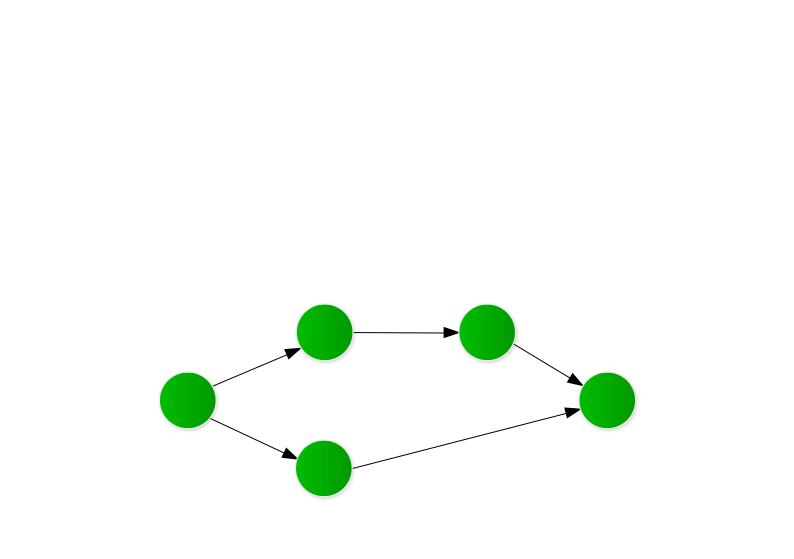
\includegraphics[width=0.85\textwidth]{images/mspsp1.png}}%
	\only<3>{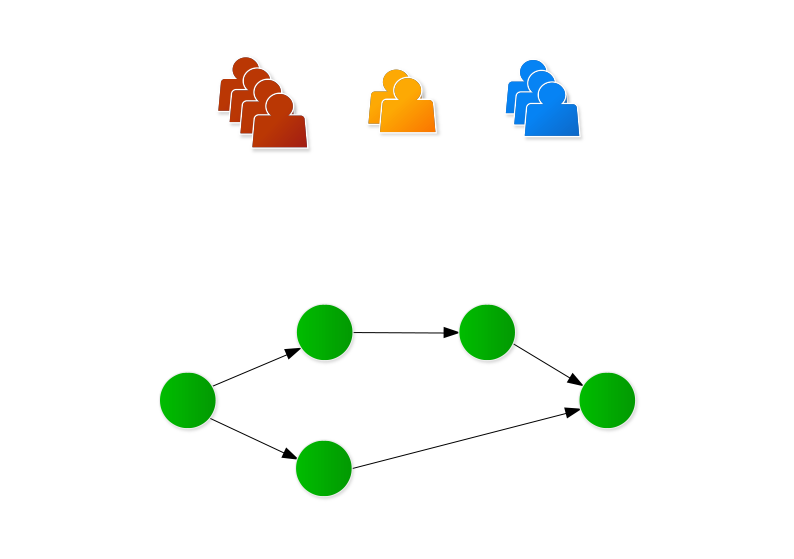
\includegraphics[width=0.85\textwidth]{images/mspsp2.png}}%
	\only<4>{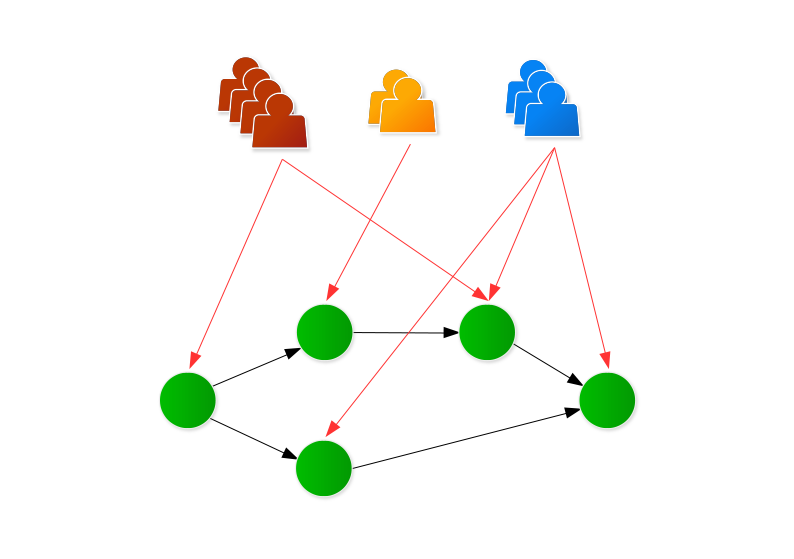
\includegraphics[width=0.85\textwidth]{images/mspsp3.png}}%
	\only<5>{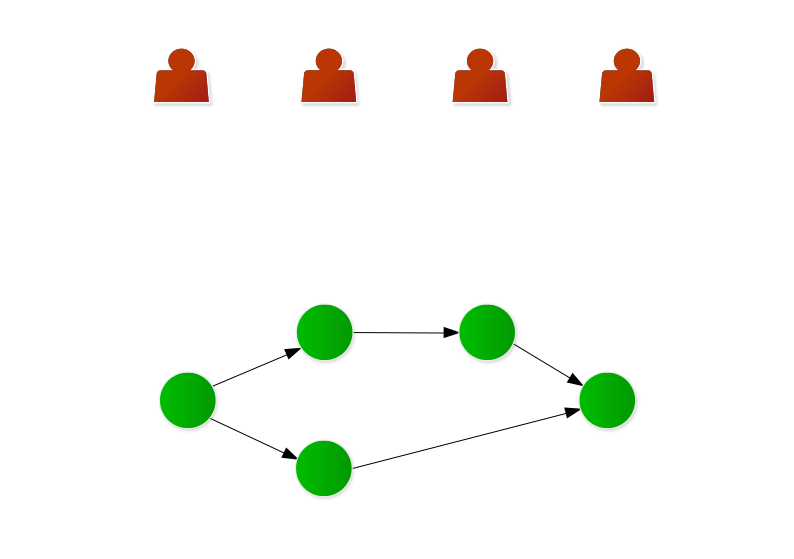
\includegraphics[width=0.85\textwidth]{images/mspsp4.png}}%
	\only<6>{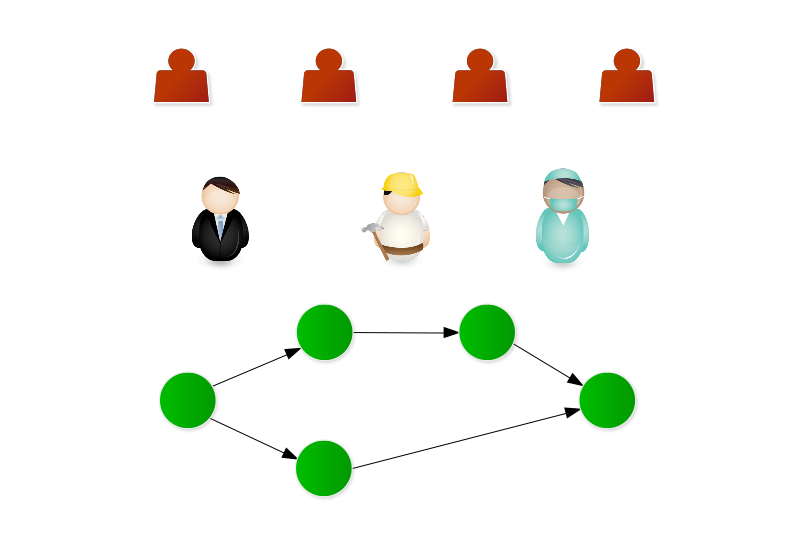
\includegraphics[width=0.85\textwidth]{images/mspsp5.png}}%
	\only<7>{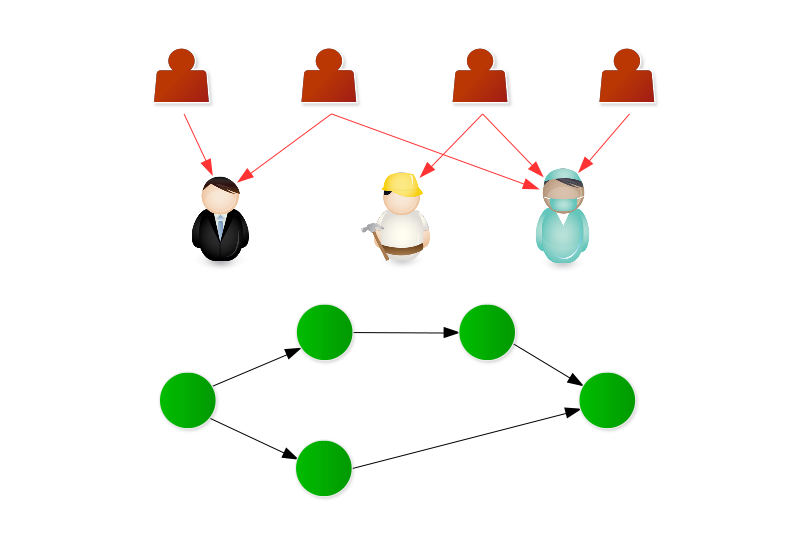
\includegraphics[width=0.85\textwidth]{images/mspsp6.png}}%
	\only<8>{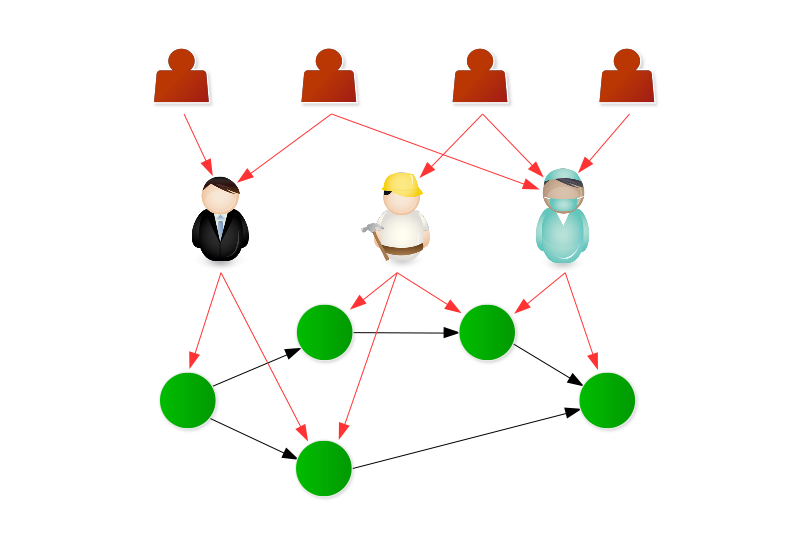
\includegraphics[width=0.85\textwidth]{images/mspsp7.png}}%
\end{figure}%
\end{frame}

\subsection{Example}
\begin{frame}{Intro: Example}
	\scriptsize
	\begin{multicols}{2}
		\begin{table}
			\caption{Workers' Skills}
			\vspace{-3mm}
			\begin{tabular}{ccccc}
				\toprule
				 & Alice & Bob & Carl & Dora \\\midrule\midrule
				{\tiny {\bf Programmer}} & - & \checkmark & \checkmark & \checkmark \\
				{\tiny {\bf DB Designer}} & \checkmark & - & - & - \\
				{\tiny {\bf Webmaster}} & \checkmark & \checkmark & - & \checkmark \\
				\bottomrule
			\end{tabular}
		\end{table}\pause
		\begin{figure}[H]
			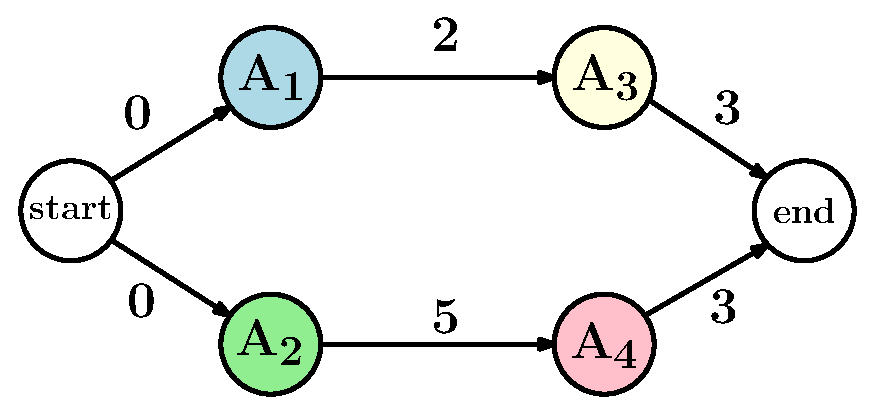
\includegraphics[width=\linewidth]{images/precgraph.eps}
			\caption{Precedence Graph}
		\end{figure}\pause
		\columnbreak

		\begin{table}
			\caption{Skill Requirement}
			\begin{tabular}{ccccc}
				\toprule
				 & $A_1$ & $A_2$ & $A_3$ & $A_4$ \\\midrule\midrule
				{\tiny {\bf Programmer}} & - & 1 & 2 & 1 \\
				{\tiny {\bf DB Designer}} & 1 & - & - & 1 \\
				{\tiny {\bf Webmaster}} & 1 & 1 & - & - \\
				\bottomrule
			\end{tabular}
		\end{table}\pause
		\vspace{-8mm}
		\begin{figure}[H]
			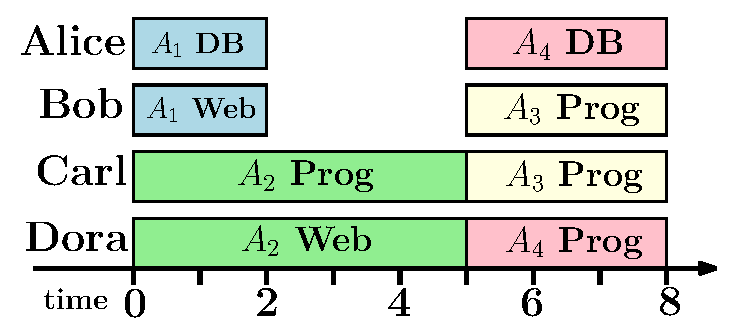
\includegraphics[width=\linewidth]{images/sched.eps}
			\caption{Schedule}
		\end{figure}

	\end{multicols}
\end{frame}

% \subsection{Constraint Programming}
% \begin{frame}{Intro: Constraint Programming}
% 	Domain propagation
% 	\begin{itemize}
% 		\item Variables have domains of possible values
% 		\item Constraints reduce the size of these domains
% 	\end{itemize}\pause
% 	Nogood learning
% 	\begin{itemize}
% 		\item Learn from failures
% 		\item Record these failures as constraints
% 		\item Use these constraints to make inferences
% 	\end{itemize}
% \end{frame}

\subsection{Previous Work}
\begin{frame}{Intro: The Literature}
	\begin{itemize}
		\item French research group
		\begin{itemize}
			\item Principal researchers: Odile Belleguez-Morineau, Emmanuel N\'{e}ron, Carlos Montoya
			\item Exact branch and bound methods
			\item Lower bounds
			\item Adapted data from PSPLib\pause
		\end{itemize}	
		\vspace{2mm}
		\item Portuguese research group
		\begin{itemize}
			\item Principal researchers: Bernardo Almeida, Isabel Correia, Francisco Saldanha-da-Gama
			\item Constructive heuristics
			\item Randomised search heuristics
			\item Generated their own instances inspired by PSPLib\pause
		\end{itemize}
		\vspace{2mm}
		\item Polish research group
		\begin{itemize}
			\item Principal researchers: Pawe\l{} Myszkowski, Marek Skowronski
			\item Randomised search heuristics
			\item Generated their own instances inspired by real-world data
		\end{itemize}
	\end{itemize}
\end{frame}

% \begin{frame}{Intro: Timeline of the Literature}
% 	\begin{itemize}
% 		\item \color{red}{French} 
% 		\item \color{blue}{Portuguese} 
% 		\item \color{green}{Polish} 
% 		\item \color{darkgray}{Other} 
% 	\end{itemize}
% 	\begin{figure}[H]
% 		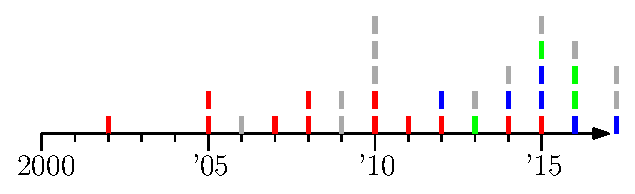
\includegraphics[width=0.8\linewidth]{images/lit_timeline.eps}
% 	\end{figure}
% \end{frame}


%~~~~~~~~~~~~~~~~~~~~~~~~~~~~~~~~~~~~~~~~~~~~~~~~~~~~~~~~~~~~~~~~~~~~~~~~~~~~~~~~~%
% MODEL
\section{Modelling the MSPSP}
\subsection{Overview}
\begin{frame}{Model}
	\begin{itemize}
		\item Objective
		\begin{itemize}
			\item Minimise the total project duration\pause
		\end{itemize}
	\end{itemize}
	\vspace{5mm}
	\begin{itemize}
		\item Two main decisions\pause
		\vspace{2mm}
		\begin{enumerate}
			\item Scheduling decisions
			\begin{itemize}
				\item Activity start times\pause
			\end{itemize}
			\vspace{2mm}
			\item Assignment decisions
			\begin{itemize}
				\item Workers to activities
				\vspace{1mm}
				\item Skill contribution of workers
			\end{itemize}
		\end{enumerate}
	\end{itemize}
\end{frame}

\subsection{Constraints}
\begin{frame}{Model: Constraints Outline}
	\begin{itemize}
		\item Precedence relations are respected\pause
		\vspace{2mm}
		\item Skill requirement is satisfied
		\begin{itemize}
			\item A worker for each skill must be present to perform the activity\pause
		\end{itemize}
		\vspace{2mm}
		\item Workers perform only one activity at a time
		\begin{itemize}
			\item Also, workers cannot multi-task\pause
		\end{itemize}
		\vspace{2mm}
		\item Workers only use skills they have mastered
	\end{itemize}
\end{frame}

\begin{frame}{Model: Decision Variables}
	\begin{adjustwidth}{-.9in}{-.9in}
	\begin{table}[h]
		\centering
		\vspace{1mm}
		\begin{tabular}{llp{8cm}}
			\toprule
			\multicolumn{3}{l}{ \bf{Decision Variables}}  \\
			\midrule\midrule
			Primary & $s_i$ & Start time of activity $i \in V$ \\
			 & $y_{ir}^s$ & 1 iff resource $r \in R$ contributes with skill $s \in S$ to activity $i \in V$\\\midrule\pause
			% \multicolumn{2}{l}{\rule{0pt}{2ex} \bf{Auxilliary Decision Variables}}  \\
			Auxiliary & $o_{ij}$ & 1 iff activities $i$ and $j$ overlap for $(i,j)\in U$ \\
			 & $x_{ir}$ & 1 iff resource $r \in R$ is assigned activity $i \in V$ \\
			\bottomrule
		\end{tabular}
		\label{tab:vars}
	\end{table}
	\end{adjustwidth}
\end{frame}

\begin{frame}{Model: Basic Constraints}
	\begin{adjustwidth}{-.2in}{-.2in}
	\begin{IEEEeqnarray}{lCl}
	    s_i + p_i \leq s_j 
	    &\hspace{2mm}& \forall (i, j) \in E\nonumber\\[4mm]
	    \sum\nolimits_{r\in R} y_{ir}^s = sr_i^s
	    &\hspace{2mm}& \forall i\in V, \forall s\in S\nonumber\\[4mm]
	    \sum\nolimits_{s \in  S} \sum\nolimits_{i\in V: s_i \leq t < s_i + p_i} y_{ir}^s \leq 1 
	    &\hspace{2mm}& \forall r\in R, \forall t \in \left\{ 0,1,\ldots,\sum\nolimits_{i\in V} p_i \right\}\nonumber\\[4mm]
	    y_{ir}^s \leq mast_{rs} 
	    &\hspace{2mm}& \forall i\in V, \forall r\in R, \forall s \in S\nonumber
	\end{IEEEeqnarray}
	\end{adjustwidth}
\end{frame}

% \begin{frame}{Model: Redundant Constraints}
% 	\begin{adjustwidth}{-.2in}{-.2in}
% 	\begin{IEEEeqnarray}{CCl}
% 		\IEEEeqnarraymulticol{1}{c}{{\tt cumulative}(s,~p,~[~sr_{is}: i \in V],~|R_s|)} & & \forall s \in S\nonumber\\[6mm]
% 		\IEEEeqnarraymulticol{1}{c}{{\tt cumulative}\left(s,~p,~\left[~\sum_{s \in S} sr_{is}: i \in V~\right],~m\right)} \nonumber
% 	\end{IEEEeqnarray}
% 	\end{adjustwidth}
% \end{frame}

\begin{frame}{Model: Choice of Formulation}
	Unary Resource Constraint
	\vspace{1mm}
	\begin{itemize}
		\item Each worker only performs one activity at a time\pause
	\end{itemize}
	\vspace{5mm}
	Possible ways of modelling
	\vspace{1mm}
	\begin{enumerate}
		\item Time-indexed decomposition
		\vspace{1mm}
		\item Global constraints (either disjunctive or cumulative)
		\vspace{1mm}
		\item Order constraints
	\end{enumerate}
\end{frame}

\begin{frame}{Model: Unary Resource Constr.}
	\begin{itemize}
		\item Time-indexed decomposition
		\begin{IEEEeqnarray}{lCl}
		    \sum\nolimits_{s \in  S} \sum\nolimits_{i\in V: s_i \leq t < s_i + p_i} y_{ir}^s \leq 1 
		    &\hspace{2mm}& \forall r\in R, \forall t \in \left\{ 0,1,\ldots,\sum\nolimits_{i\in V} p_i \right\} \nonumber
		\end{IEEEeqnarray}\pause
		\vspace{3mm}
		\item Cumulative global constraint
		\begin{align}
		    & {\tt cumulative}((s_{i})_{i\in V}, (p_{i})_{i\in V}, 
		        (x_{ir})_{i\in V}, 1)
		    && \forall r\in R \nonumber
		\end{align}
	\end{itemize}
\end{frame}

\begin{frame}{Model: Unary Resource Constr.}
	\begin{itemize}
		\item $U=$ set of \emph{unrelated} activity pairs w.r.t. the precedence graph
		\item First order constraint formulation
		\begin{align}
		    \neg o_{ij} 
		    & \Leftrightarrow (s_{i} + p_{i} \leq s_{j}) \vee (s_{j} + p_{j} \leq s_{i})
		    && \forall (i, j) \in U \nonumber\\
		    (x_{ir} \wedge x_{jr}) 
		    & \Rightarrow \neg o_{ij}
		    && \forall (i, j) \in U, r\in R\nonumber
		\end{align}\pause
		\vspace{3mm}
		\item Second order constraint formulation
		\begin{multline}
		    (o_{ij} \Rightarrow s_i + p_{i} \leq s_{j}) \wedge
		    (\neg o_{ij} \Rightarrow s_{j} + p_{j} \leq s_{i})
		    \\
		    \forall (i, j) \in U, \exists s\in S: 
		        sr_{is} + sr_{js} > \sum\nolimits_{r\in R} mast_{rs}\nonumber
		\end{multline}
	\end{itemize}
\end{frame}


%~~~~~~~~~~~~~~~~~~~~~~~~~~~~~~~~~~~~~~~~~~~~~~~~~~~~~~~~~~~~~~~~~~~~~~~~~~~~~~~~~%
% DATA
\section{Data}
\begin{frame}{Data: Overview}
	\begin{itemize}
		% \pause
		\item Tested on data from the literature and generated our own data\pause
	\end{itemize}
\begin{table}[tpb]
	\begin{adjustwidth}{-0.5cm}{}
    \setlength{\tabcolsep}{3pt}
    \centering
    \small
	\begin{tabular}{@{}lrrrrrrr@{}}
		\toprule
		&  &  &  &  & \multicolumn{3}{c}{Best known results}\\ 
        \cmidrule(l){6-8} 
		set & \multicolumn{1}{l}{\#instances} & \#act. & \#skill & \#res. & \multicolumn{1}{c}{source} & \multicolumn{1}{r}{\%optimal} & {\color{red} \#unsolved} \\ \midrule\midrule
		1a     & 216 & 22 & 4 & 10-30 & Correia et al. 2012 & 93.98 & {\color{red} 13}\\
		1b     & 216& 42 & 4 & 20-60 & Almeida et al. 2016 & 2.31 & {\color{red} 211} \\ \midrule\pause
		2a     & 110 & 20-51 & 2-8 & 5-14 & Montoya et al. 2014 & 43.64 & {\color{red} 62} \\
		2b     & 77 & 32-62 & 9-15 & 5-19 & Montoya et al. 2014 & 66.20 & {\color{red} 24} \\
		2c     & 91 & 22-32 & 3-12 & 4-15 & Montoya et al. 2014 & 51.11 & {\color{red} 44} \\ \midrule\midrule\pause
		& {\bf 710} & {\bf 20-62} & {\bf 2-15} & {\bf 4-60} & & & {\bf {\color{red} 354}} \\\bottomrule
	\end{tabular}
    \end{adjustwidth}
	\label{tab:data}
\end{table}
		% \begin{itemize}
		% 	\item equivalent to the Portuguese group's data\pause
		% \end{itemize}
	% 	\vspace{2mm}
	% 	\item Small data set: 216 unique instances
	% 	\begin{itemize}
	% 		\item 20 activities
	% 		\vspace{1mm}
	% 		\item 4 skills
	% 		\vspace{1mm}
	% 		\item 10-30 workers\pause
	% 		\vspace{1mm}
	% 		\item \alert{13 unsolved}\pause
	% 	\end{itemize}
	% 	\vspace{2mm}
	% 	\item Large data set: 216 unique instances
	% 	\begin{itemize}
	% 		\item 40 activities
	% 		\vspace{1mm}
	% 		\item 4 skills
	% 		\vspace{1mm}
	% 		\item 20-60 workers\pause
	% 		\vspace{1mm}
	% 		\item \alert{211 unsolved}
	% 	\end{itemize}
\end{frame}

\begin{frame}{Data: Complexity Measures}
	\begin{enumerate}
		\item Skill Factor
		\vspace{1mm}
		\begin{itemize}
			\item $SF \in \{1,~0.75,~0.5,~variable\}$\pause
		\end{itemize}
		\vspace{2mm}
		\item Network Complexity
		\vspace{1mm}
		\begin{itemize}
			\item $NC \in \{1.5,~1.8,~2.1\}$\pause
		\end{itemize}
		\vspace{2mm}
		\item Modified Resource Strength
		\vspace{1mm}
		\begin{itemize}
			\item varied over 3 values
			\item \[MRS=\frac{m}{\sum_{i\in V}\sum_{s \in S}sr_{is}}\]
		\end{itemize}
	\end{enumerate}
	% \vspace{3mm}
	% Therefore, 36 types of instances 
\end{frame}


%~~~~~~~~~~~~~~~~~~~~~~~~~~~~~~~~~~~~~~~~~~~~~~~~~~~~~~~~~~~~~~~~~~~~~~~~~~~~~~~~~%
% EXPERIMENTS
\section{Experiments}

\subsection{Results}
\begin{frame}{Experiments: Search Strategies}

	\begin{itemize}
		\item Basic Search
		\begin{itemize}
			\item  Start times ($s_i$)
		\end{itemize}\pause
			\vspace{2mm}
		\item Sequential Searches
		\begin{itemize}
			\item Start times ($s_i$), then worker assignment ($x_{ir}$)
			\item Start times ($s_i$), then contribution of each worker ($y_{ir}^s$)\pause
			\begin{itemize}
				\item leads to bad branching decisions early in the search tree\pause
			\end{itemize}
		\end{itemize}
		\item More involved sequential search $\Rightarrow$ mostly avoids previous problem
		\begin{itemize}
			\item Start time and worker contribution of activity 1 ($s_1,~y_{1r}^s$)
			\item Start time and worker contribution of activity 2 ($s_2,~y_{2r}^s$)
			\item $\vdots$
			\item Start time and worker contribution of activity n ($s_n,~y_{nr}^s$)
		\end{itemize}
	\end{itemize}
\end{frame}

\begin{frame}{Experiments: Search Strategies}
	\begin{itemize}
		\item Priority search $\Rightarrow$ Group scheduling and assignment decisions of each activity together\vspace{2mm}\pause
		\begin{itemize}
			\item {\tt priority-ff}: choose activity group by smallest start time domain \vspace{2mm}
			\item {\tt priority-sml}: choose activity group by smallest largest possible start time\vspace{2mm}
			\item {\tt priority-sm}: choose activity group by smallest possible start time\pause
		\end{itemize}
		\item For more details see: Feydy et al. 2017, \emph{Priority Search with MiniZinc}, ModRef2017
	\end{itemize}
\end{frame}


\begin{frame}{Experiments: Set 1'a}
	\begin{itemize}
		\item Tested on 216 generated instances with 22 activities 
		\item Time limit of 600 seconds
		\item Solver used is {\tt Chuffed}
	\end{itemize}
	\begin{table}[tpb]
	\begin{adjustwidth}{-.9in}{-.9in}
    \centering
    \small
    \begin{tabular}{llrrr}
        \toprule
        unary cons. & search & \#nodes & \%optimal & runtime   \\
        \midrule\midrule
        cumulative & default & 370,174 & 100.00 & 10.23s \\
        order-1 & default & 97,085 & 100.00 & 2.73s \\
        order-2 & default & 54,282 & 100.00 & 1.30s \\
        \midrule\pause
        order-2 & {\tt priority-ff}    & 41,762 & 100.00 & 1.25s \\
        order-2 & {\tt priority-sml}    & 20,786 & 100.00 & 0.68s \\
        order-2 & {\tt priority-sm}    & 13,241 & 100.00 & {\color{red} {\bf 0.51s} }\\
        \bottomrule
    \end{tabular}
	\end{adjustwidth}
    \label{tab:resultsSet1a}
\end{table}
\end{frame}

\begin{frame}{Experiments: Set 2 and Set 1'b}
	\begin{itemize}
		\item Tested on remaining benchmark instances\pause
	\end{itemize}
	\begin{table}[ptb]
		\begin{adjustwidth}{-.3in}{-.3in}
		\setlength{\tabcolsep}{5pt}
		\small
		\begin{tabular}{lrrrrrrrr}
			\toprule
			set & \#nodes & \%gap & \#opt & \%opt & mean runtime & {\color{red} \#prev. open} & {\color{red} \#closed} \\
			\midrule\midrule
			$2a$ & 2,223k & 185.2 & 81/110 & 73.6 & 195.2s & {\color{red} 62} & {\color{red} $\geq$33 } \\\pause
			$2b$ & 816k & 22.4 & 63/77 & 81.8 & 122.9s & {\color{red} 24} & {\color{red} $\geq$10 } \\\pause
			$2c$ & 14k & 0.0 & 91/91 & 100.0 & 1.2s & {\color{red} 44} & {\color{red} 44 } \\\midrule\pause
			$1'b$ & 7,584k & 49.3 & 27/216 & 12.5 & 534.6s & {\color{red} ``211''} & {\color{red} --} \\
			\bottomrule
		\end{tabular}
		\label{tab:benchmarks}
		\end{adjustwidth}
	\end{table}
\end{frame}

\begin{frame}{Experiments: Complexity Measures}
	\begin{itemize}
		\item Results of set $1'b$\pause
	\end{itemize}
	\begin{table}[H]
		\begin{adjustwidth}{-.9in}{-.9in}
			\centering
			\scriptsize
			\begin{tabular}{llrrrrrr}
				\toprule
				measure & value  & \#nodes & \#props & \%gap & \#opt & \%opt &  runtime(s) \\
				\midrule\midrule
				SF & 1 & 5.9m & 706k & 48.1 & 6/54 & 11.1 & 535.5 \\
				 & 0.75 & 8.9m & 765k & 51.8 & 4/54 & 7.4 & 559.9 \\
				 & 0.5 & 6.7m & 914k & 44.1 & 12/54 & 22.2 & 489.7 \\
				 & variable & 8.6m & 754k & 52.4 & 5/54 & 9.26 & 553.5 \\\midrule
				NC & 1.5 & 7.7m & 872k & 58.3 & 6/72 & 8.3 & 559.9 \\
				 & 1.8 & 7.9m & 812k & 47.7 & 8/72 & 11.1 & 541.3 \\
				 & 2.1 & 7.0m & 671k & 41.03 & 13/72 & 18.1 & 502.8 \\\midrule
				MRS & \#1 & 7.4m & 1,106k & 79.2 & 11/72 & 15.3 & 525.4 \\
				 & \#2 & 7.9m & 734k & 45.6 & 6/72 & 8.3 & 558.4 \\
				 & \#3 & 7.3m & 515k & 24.0 & 10/72 & 13.9 & 520.1 \\\midrule
				Overall &  & 7.5m & 785k & 49.3 & 27/216 & 12.5 & 534.6 \\\bottomrule
			\end{tabular}
		\end{adjustwidth}
	\end{table}
\end{frame}

\begin{frame}{MSPSP Instance Library}
	\begin{itemize}
		% \pause
		\item All instances have been made available at \url{https://github.com/youngkd/MSPSP-InstLib}
	\end{itemize}
	\begin{figure}%
		\centering%
		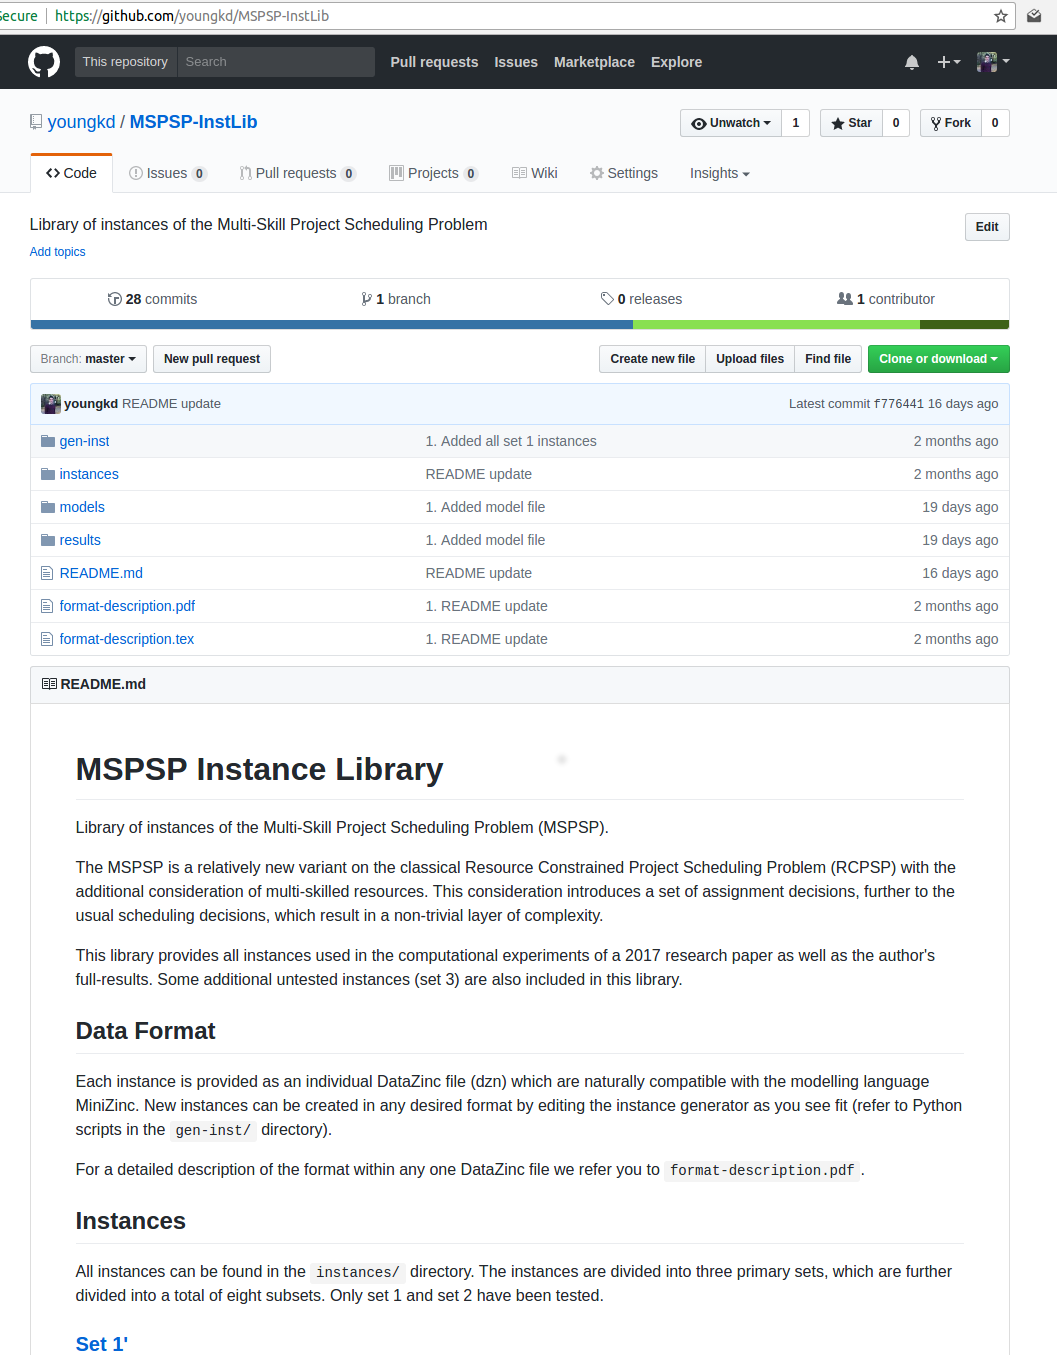
\includegraphics[width=0.7\textwidth]{images/lib-shot.png}%
	\end{figure}%
\end{frame}

% \begin{frame}{Experiments: Large Data Set}
% 	\begin{itemize}
% 		\item Time limit of 3600 seconds \pause
% 	\end{itemize}
% 	\begin{table}[H]
% 		\begin{adjustwidth}{-.9in}{-.9in}
% 			\centering
% 			\scriptsize
% 			\vspace{2mm}
% 			\begin{tabular}{cc|rrrrrrrr}
% 				\hline
% 				measure & value  & \#nodes & \#props & \%gap & \#opt & \%opt & opt rt. &  total rt. \\
% 				\hline SF & 1 & 36m & 4,254m & 48.35 & 7 & 12.96 & 257.55 & 3166.72 \\
% 				 & 0.75 & 47m & 4,296m & 49.63 & 4 & 7.41 & 545.44 & 3373.74 \\
% 				 & 0.5 & 32m & 4,468m & 42.06 & 20 & 37.04 & 782.20 & 2556.37 \\
% 				 & var & 45m & 4,302m & 49.82 & 5 & 9.26 & 130.97 & 3278.79 \\\hline
% 				NC & 1.5 & 41m & 5,007m & 57.33 & 8 & 11.11 & 819.48 & 3291.05 \\
% 				 & 1.8 & 42m & 4,381m & 46.09 & 11 & 15.28 & 558.06 & 3135.26 \\
% 				 & 2.1 & 36m & 3,602m & 38.99 & 17 & 23.61 & 446.41 & 2855.40 \\\hline
% 				MRS & \#1 & 37m & 6,083m & 76.93 & 14 & 19.44 & 327.52 & 2963.68 \\
% 				 & \#2 & 42m & 4,154m & 43.36 & 8 & 11.11 & 913.89 & 3301.54 \\
% 				 & \#3 & 39m & 2,753m & 23.94 & 14 & 19.44 & 599.07 & 3016.49 \\\hline
% 				\hline \bf{Overall} &  & \bf{40m} & \bf{4,330m} & \bf{47.92} & \alert{\bf{36}} & \bf{16.67} & \bf{563.43} & \bf{3093.90} \\\hline\hline
% 			\end{tabular}
% 		\end{adjustwidth}
% 	\end{table}
% \end{frame}

%~~~~~~~~~~~~~~~~~~~~~~~~~~~~~~~~~~~~~~~~~~~~~~~~~~~~~~~~~~~~~~~~~~~~~~~~~~~~~~~~~%
% CONCLUSION
\section{Conclusion}
\subsection{Summary}
\begin{frame}{Summary}
	\begin{itemize}
		\item Applied the constraint programming solver {\tt Chuffed} to the MSPSP\pause
		\vspace{2mm}
		\item Generated a set of benchmark instances\pause
		\vspace{2mm}
		\item Created an effective constraint programming model\vspace{2mm}
		\begin{itemize}
			\item Together with an application tailored search strategy
		\end{itemize}
	\end{itemize}
\end{frame}

% \subsection{Future Work}
% \begin{frame}{Future Work}
% 	\begin{itemize}
% 		\item Apply activity-based search to the large dataset\pause
% 		\vspace{2mm}
% 		\item Create a more structured search procedure in chuffed
% 	\end{itemize}
% \end{frame}

\begin{frame}{Acknowledgements}
	\begin{itemize}
		\item Dr. Andreas Schutt
		\vspace{2mm}
		\item Dr. Thibaut Feydy
		\vspace{2mm}
		\item Adrian Goldwaser
	\end{itemize}
\end{frame}

\begin{frame}{}
	\centering
	{\Large Thanks for listening!\vspace{1cm}\\
	Questions?}
\end{frame}

\end{document}
